\chapter{Classification à quatre maisons}
\label{ch:classifieur}

\begin{lecture}
Le modèle construit jusqu'ici répond à une seule question : \Gryf ou non.
Or le problème en compte quatre, dont une réponse unique doit sortir. Pour cela,
la construction réutilise les outils déjà en place : le même ajustement est répété
pour chaque maison, et les quatre scores obtenus sont comparés.
\end{lecture}

\section{Un modèle par maison}

Le modèle construit jusqu'ici répond par oui ou par non, parce qu'une frontière
sépare le plan en deux régions et pas davantage. Quatre maisons demandent une
autre construction, et deux voies s'offrent.

La première consiste à concevoir un modèle qui produise directement quatre
probabilités de somme $1$ : c'est la régression \emph{softmax}, dont la
dérivation diffère de celle menée aux chapitres précédents. La seconde ramène le
problème à quatre questions binaires, chacune traitée par le modèle déjà en
place, puis combine les quatre réponses. C'est cette seconde voie qui est
retenue, parce qu'elle réemploie tout ce qui précède sans y changer une ligne.

Elle porte le nom d'\emph{un contre tous}, ou \emph{one-vs-rest}. Pour chaque
maison, on reprend le procédé à l'identique, seule la cible changeant :
\[
  y_i=1 \text{ si l'élève } i \text{ appartient à la maison traitée},\qquad
  y_i=0 \text{ sinon.}
\]
Les notes et leur préparation sont inchangées, le tableau $\X$ est le même pour
les quatre modèles ; seule la colonne des réponses change.

\begin{figure}[htbp]
\centering
\begin{tikzpicture}[
  cell/.style={draw=ink!25,minimum width=22mm,minimum height=5.6mm,
    font=\scriptsize,inner sep=1.5pt},
  bit/.style={draw=ink!25,minimum width=8mm,minimum height=5.6mm,
    font=\scriptsize,inner sep=1.5pt},
  head/.style={font=\scriptsize\bfseries,text=ink,align=center}]

\node[cell,fill=gryff!12] (m1) {\Gryf};
\node[cell,fill=slyth!12,below=0.5mm of m1] (m2) {\Slyth};
\node[cell,fill=raven!12,below=0.5mm of m2] (m3) {\Rav};
\node[cell,fill=huffle!12,below=0.5mm of m3] (m4) {\Huff};
\node[head,above=2.5mm of m1] {maison};

\foreach \k/\dx/\col/\a/\b/\c/\d in {%
  1/3.2/gryff/1/0/0/0, 2/4.5/huffle/0/0/0/1,
  3/5.8/raven/0/0/1/0, 4/7.1/slyth/0/1/0/0}{
  \node[bit,fill=\col!14] (a\k) at ($(m1)+(\dx,0)$) {$\a$};
  \node[bit,fill=\col!14] (b\k) at ($(m2)+(\dx,0)$) {$\b$};
  \node[bit,fill=\col!14] (c\k) at ($(m3)+(\dx,0)$) {$\c$};
  \node[bit,fill=\col!14] (d\k) at ($(m4)+(\dx,0)$) {$\d$};
}
\node[head,text=gryff,above=2.5mm of a1] {$y^{(G)}$};
\node[head,text=huffle,above=2.5mm of a2] {$y^{(H)}$};
\node[head,text=raven,above=2.5mm of a3] {$y^{(R)}$};
\node[head,text=slyth,above=2.5mm of a4] {$y^{(S)}$};
\end{tikzpicture}
\caption{Quatre colonnes de réponses construites depuis la même colonne de
maisons. Chaque ligne porte exactement un $1$ : les quatre modèles sont ajustés
séparément, mais leurs cibles restent liées par cette contrainte, qu'aucun d'eux
ne connaît.}
\label{fig:quatre-cibles}
\end{figure}
\FloatBarrier

Quatre descentes indépendantes donnent quatre jeux de coefficients. Sur les
deux matières employées ici :

\begin{table}[htbp]
\centering
\begin{tabular}{lrrr}
\toprule
maison traitée & $w_0$ & $w_1$ (\Herb) & $w_2$ (\Runes) \\
\midrule
\Gryf & $-4{,}997$ & $-3{,}625$ & $+3{,}655$ \\
\Huff & $-3{,}056$ & $+3{,}889$ & $-4{,}358$ \\
\Rav  & $-3{,}729$ & $+4{,}061$ & $+3{,}869$ \\
\Slyth  & $-4{,}545$ & $-3{,}341$ & $-3{,}549$ \\
\bottomrule
\end{tabular}
\caption{Les quatre modèles binaires. Chaque maison correspond à un couple de
signes distinct, et les quatre combinaisons possibles sont occupées.}
\label{tab:quatre}
\end{table}

Ces douze nombres se lisent sur le nuage par le procédé du
chapitre~\ref{ch:modele} : le signe de $w_1$ dit de quel côté en \Herb se
trouve la maison traitée, celui de $w_2$ fait de même en \Runes. Les quatre
maisons occupant chacune un coin du nuage, les quatre couples de signes possibles
se trouvent employés, un par maison.

Les quatre biais sont négatifs pour une raison commune : chaque maison est
minoritaire face aux trois autres réunies, si bien qu'un élève pris au hasard
reçoit un score négatif dans les quatre modèles.

\section{Règle du score maximal}

Un nouvel élève reçoit quatre scores, un par maison, et il faut en tirer une
réponse. Chaque score mesure à quel point son modèle penche pour sa maison :
retenir le plus élevé est la règle la plus directe.
\[
  \text{maison prédite}=\arg\max_{k}\ z_k,
  \qquad z_k=w_{k0}+w_{k1}x_1+w_{k2}x_2
\]

Cette règle repose sur une hypothèse qu'il vaut mieux énoncer : que les quatre
scores soient comparables entre eux. Rien ne l'assure a priori, les quatre
modèles ayant été ajustés séparément, chacun sur sa propre question. Deux
éléments la rendent acceptable ici. Tous partagent la même famille de fonctions et les mêmes notes standardisées,
donc la même échelle d'entrée ; et la sigmoïde, croissante et identique pour tous, convertit chaque
score en probabilité de la même manière, si bien que comparer les scores ou les
probabilités donne la même réponse. La décision se prend sur les scores, et les
probabilités ne se calculent que pour être affichées.

Un seuil de $0{,}5$ appliqué séparément à chaque modèle produirait un autre
résultat : il pourrait ne désigner aucune maison, si les quatre probabilités
tombaient en dessous, ou plusieurs à la fois. La règle du maximum désigne
toujours exactement une maison, quelle que soit la valeur des scores.

\begin{releve}
L'élève $3$, de notes standardisées $x_1=-1{,}485$ et $x_2=+0{,}275$, donne
\begin{align*}
  z_G &= -4{,}997-3{,}625\times(-1{,}485)+3{,}655\times0{,}275 = +1{,}393,\\
  z_H &= -3{,}056+3{,}889\times(-1{,}485)-4{,}358\times0{,}275 = -10{,}031,\\
  z_R &= -3{,}729+4{,}061\times(-1{,}485)+3{,}869\times0{,}275 = \phantom{0}-8{,}697,\\
  z_S &= -4{,}545-3{,}341\times(-1{,}485)-3{,}549\times0{,}275 = \phantom{0}-0{,}558.
\end{align*}
\end{releve}

Le maximum est $z_G$, et la maison prédite est celle de l'élève. Le deuxième score se tient près de deux unités en dessous.

\begin{table}[htbp]
\centering
\begin{tabular}{crrrrl}
\toprule
élève & $z_G$ & $z_H$ & $z_R$ & $z_S$ & prédiction \\
\midrule
$3$   & $\mathbf{+1{,}393}$ & $-10{,}031$ & $-8{,}697$ & $-0{,}558$
      & \Gryf, sa maison \\
$571$ & $-6{,}829$ & $-1{,}125$ & $\mathbf{-1{,}046}$ & $-6{,}781$
      & \Rav, alors qu'il est \Huff \\
\bottomrule
\end{tabular}
\caption{Deux élèves passés aux quatre modèles ; le score retenu est en gras.
L'élève $571$ départage \Rav et \Huff sur un écart de $0{,}079$, et la règle se
trompe. Ses quatre scores sont négatifs, ce qui signifie que les quatre modèles
binaires répondent « non » : le maximum reste le moins mauvais des quatre.}
\label{tab:deux-eleves}
\end{table}

\begin{figure}[htbp]
\centering
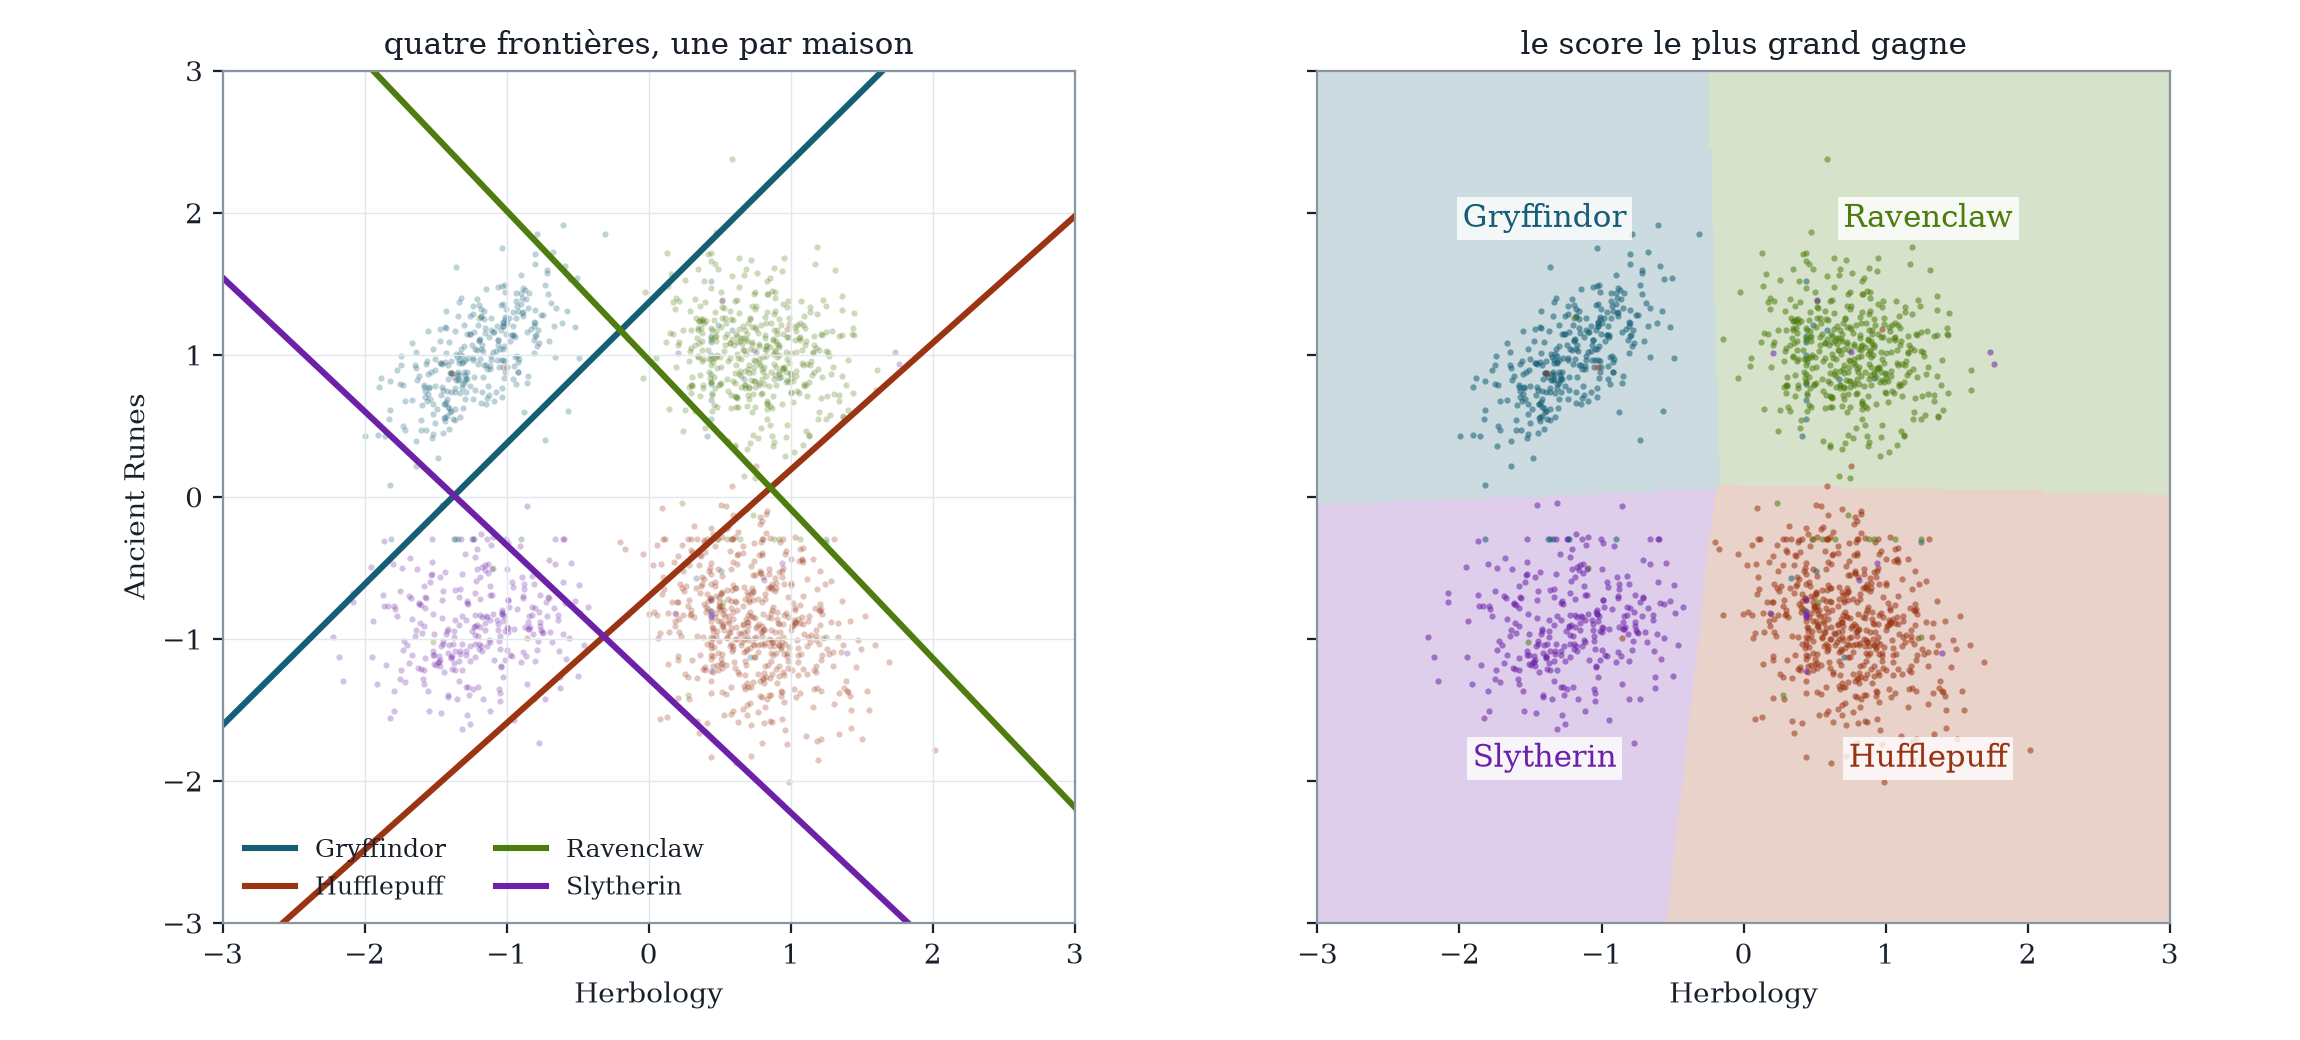
\includegraphics[width=\textwidth]{figures/regions_ovr.png}
\caption{À gauche, les quatre frontières, chacune séparant une maison des trois
autres. À droite, le découpage du plan qui en résulte : chaque point reçoit la
maison dont le score est le plus élevé. Les limites de ces quatre régions ont
leur propre direction, établie à la section suivante.}
\label{fig:regions}
\end{figure}
\FloatBarrier

\section{Forme des régions}

La règle du maximum attribue une maison à chaque point du plan. Quelle forme
prend alors l'ensemble des points attribués à une maison donnée ?

Prenons \Gryf. Son modèle l'emporte en un point lorsque son score y dépasse les
trois autres, ce qui fait trois conditions distinctes. La première s'écrit
\[
  z_G\geq z_H
  \iff
  (w_{G0}-w_{H0})+(w_{G1}-w_{H1})x_1+(w_{G2}-w_{H2})x_2\geq 0 ,
\]
et les deux autres s'obtiennent en remplaçant $H$ par $R$ puis par $S$. Le membre
de droite est une fonction affine des deux notes ; l'inégalité définit un
demi-plan, bordé par la droite où les deux scores s'égalisent.

\begin{figure}[htbp]
\centering
\makebox[\textwidth][c]{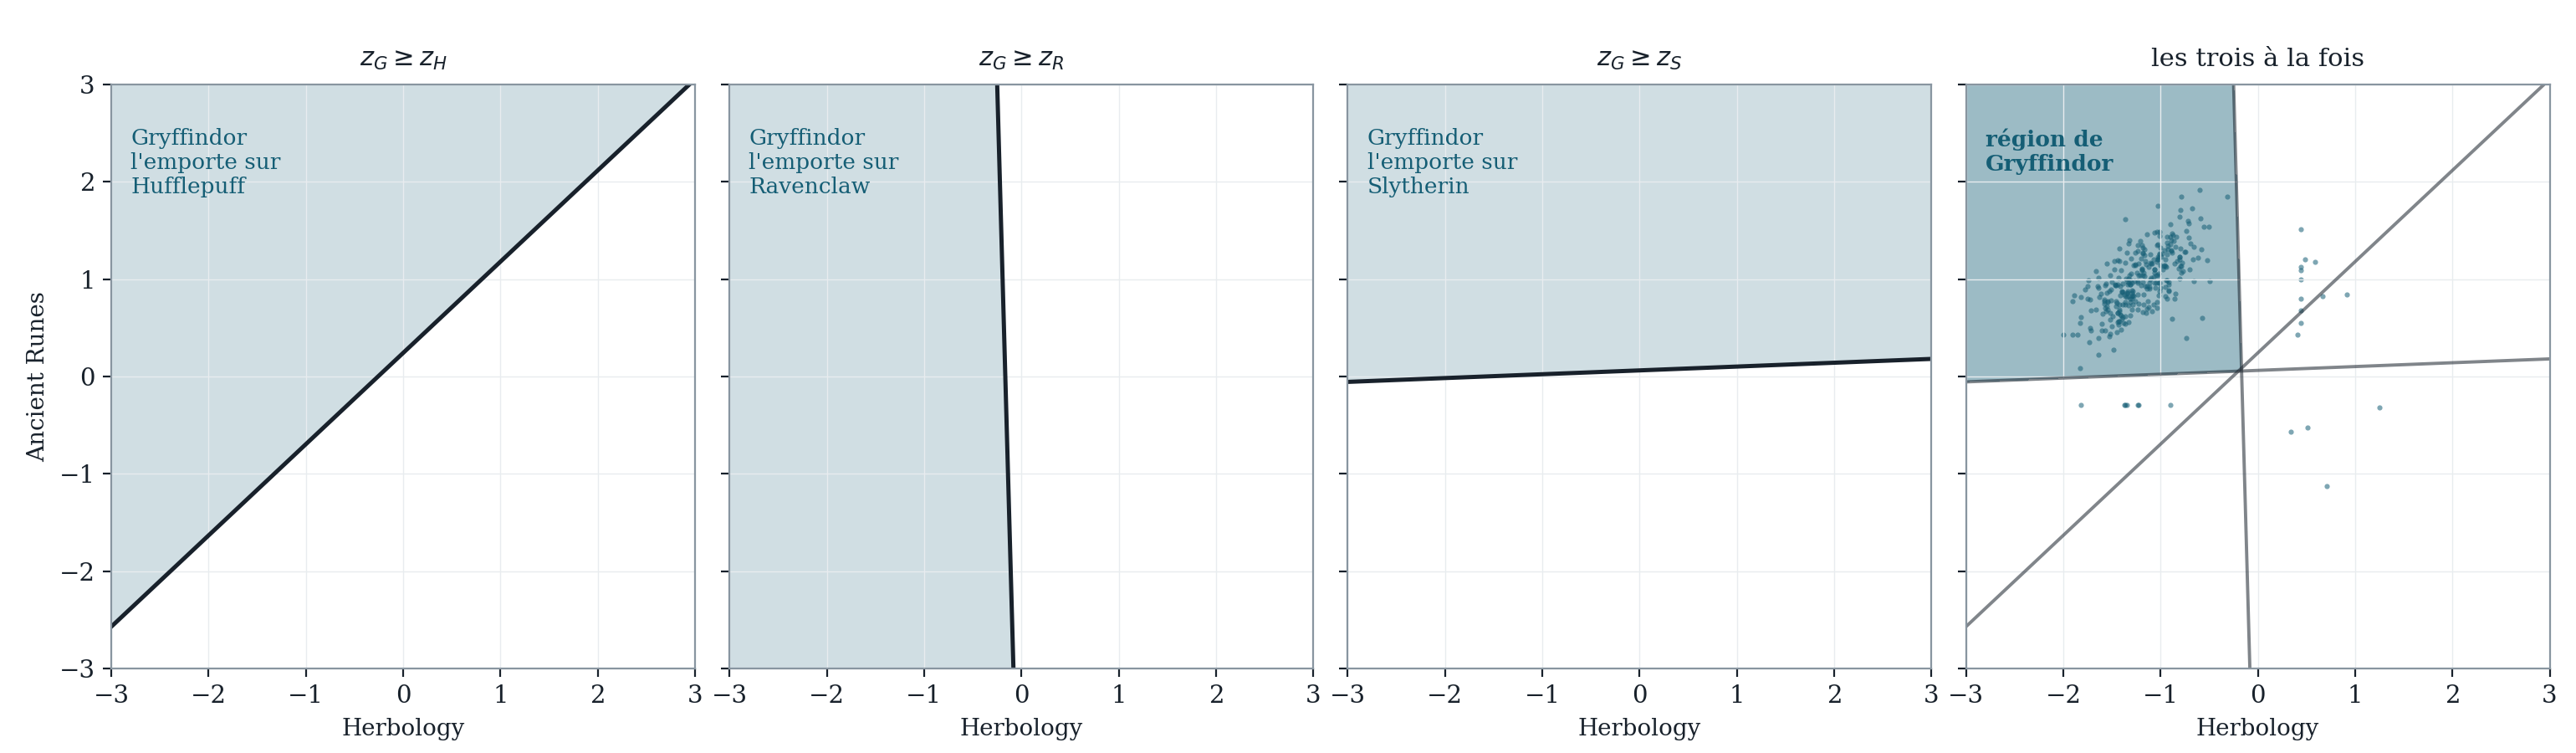
\includegraphics[width=1.18\textwidth]{figures/demiplans.png}}
\caption{Les trois demi-plans où \Gryf l'emporte sur chacun de ses rivaux, puis
leur intersection. Le dernier panneau porte les élèves de la maison, qui s'y
trouvent presque tous.}
\label{fig:demiplans}
\end{figure}
\FloatBarrier

La région de \Gryf est l'intersection de ces trois demi-plans, donc un polygone
convexe, éventuellement non borné. Trois propriétés en découlent directement.
Portés par les droites d'égalité $z_G=z_j$, ses bords se distinguent des quatre
frontières binaires du début de chapitre. Chacun s'interrompt là où un troisième
modèle prend le dessus, ce qui donne des arêtes de longueur finie. Et
deux élèves d'une même région ont tout le segment qui les joint dans cette
région, propriété de convexité qui interdit à une maison d'occuper deux zones
séparées.

Les quatre droites du début de chapitre ne disparaissent pas pour autant : la
droite $z_k=0$ sépare les points où le modèle $k$ répond « oui » de ceux où il
répond « non », tandis que la décision finale compare les quatre scores entre
eux. Ces deux questions sont différentes, et leurs droites aussi.

\begin{figure}[htbp]
\centering
\begin{tikzpicture}[x=1.28cm,y=1.28cm,font=\footnotesize]
\begin{scope}
\clip (-3,-3) rectangle (3,3);
\fill[gryff!7]  (-3,-3) -- (-0.082,-3) -- (-0.248,3) -- (-3,3) -- cycle;
\fill[raven!7]  (-0.082,-3) -- (3,-3) -- (3,3) -- (-0.248,3) -- cycle;
\draw[gridgray!35] (-3,-3) grid[step=1] (3,3);
\draw[gryff,very thick] (-3,-1.611) -- (3,4.343);
\draw[raven,very thick] (-3,4.114) -- (3,-2.186);
\draw[ink,ultra thick] (-0.082,-3) -- (-0.248,3);
\draw[ink,-{Stealth[length=2.4mm]},thick]
  (-0.197,1.171) -- ++(-0.99,-0.028);
\end{scope}
\draw[ink!45] (-3,-3) rectangle (3,3);
\draw[ink!45] (-3,0) -- (3,0);   \draw[ink!45] (0,-3) -- (0,3);
\fill[white] (-0.197,1.171) circle (2.1pt);
\draw[ink,thick] (-0.197,1.171) circle (2.1pt);
\node[gryff,anchor=west,fill=white,inner sep=1pt] at (-2.95,-1.95) {$z_G=0$};
\node[raven,anchor=east,fill=white,inner sep=1pt] at (2.95,-1.95) {$z_R=0$};
\node[ink,anchor=south,fill=white,inner sep=1.5pt] at (-0.16,3.02)
  {$z_G=z_R$};
\node[ink,anchor=south east,font=\scriptsize] at (-1.20,1.22)
  {$w_G-w_R$};
\node[gryff!85,anchor=west] at (-2.9,2.3) {$z_G>z_R$};
\node[raven!85,anchor=east] at (2.9,2.3) {$z_R>z_G$};
\node[anchor=north] at (0,-3.15) {\Herb};
\node[anchor=south,rotate=90] at (-3.15,0) {\Runes};
\end{tikzpicture}
\caption{Les deux frontières binaires de \Gryf et de \Rav, et la limite qui
sépare effectivement leurs deux régions. Cette limite a sa propre direction,
portée par le vecteur normal $w_G-w_R$, et passe par le point d'intersection des
deux premières : en ce point les deux scores valent $0$, donc ils sont égaux.}
\label{fig:limite-paire}
\end{figure}
\FloatBarrier

Quatre maisons forment six paires, donc six droites d'égalité, dont chacune ne
borde une région que sur la portion où le score commun aux deux maisons dépasse
aussi les deux autres. C'est la règle du maximum, et elle seule, qui attribue à
chaque point du plan exactement une maison, alors que les quatre modèles
s'ignorent.

Cette construction se vérifie le long d'un trajet : chaque score y devient une
fonction affine du chemin parcouru, donc une droite, et le maximum des quatre une
ligne brisée dont les points anguleux marquent les changements de région.

\begin{figure}[htbp]
\centering
\makebox[\textwidth][c]{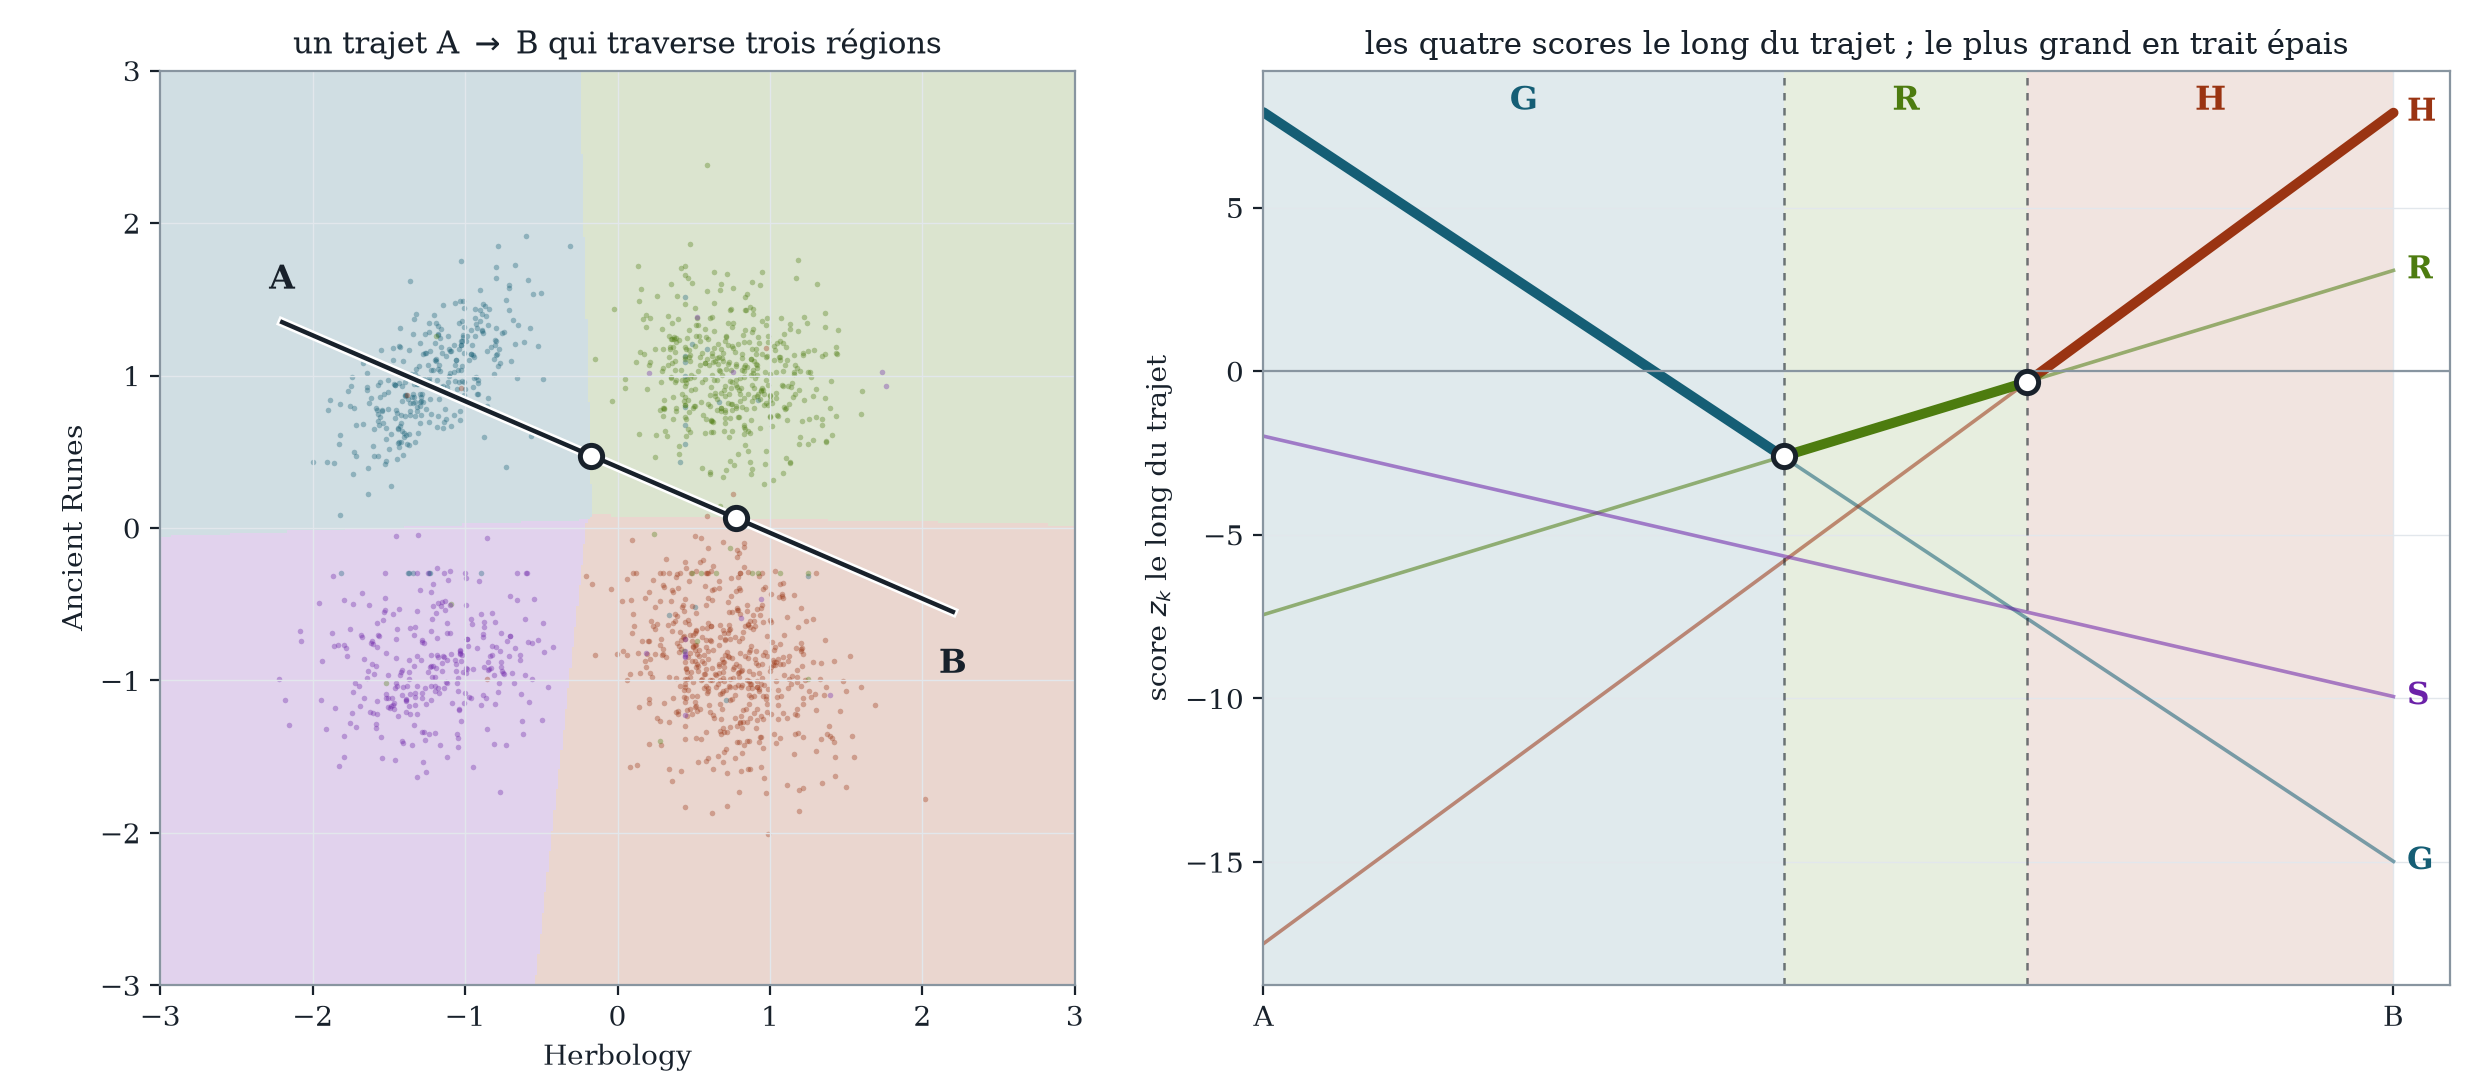
\includegraphics[width=1.2\textwidth]{figures/score_max.png}}
\caption{Le trajet du panneau de gauche part du groupe des \Gryf et rejoint celui
des \Huff. À droite, les quatre scores relevés le long de ce trajet. Le maximum
des quatre est la ligne brisée en trait épais : elle appartient à \Gryf sur le
premier tiers, à \Rav ensuite, à \Huff pour finir. Les deux points anguleux sont
les endroits où deux scores s'égalisent, et ce sont eux qui marquent le passage
d'une région à la suivante.}
\label{fig:score-max}
\end{figure}
\FloatBarrier
\section{Contenu du classifieur}

Avec dix matières au lieu de deux, chaque modèle a onze coefficients au lieu de
trois, sans autre modification. Le classifieur complet se réduit alors à :

\begin{figure}[htbp]
\centering
\begin{tikzpicture}[font=\footnotesize,
  cell/.style={draw=ink!25,minimum width=9mm,minimum height=5.4mm,
    font=\scriptsize,inner sep=1pt},
  head/.style={font=\scriptsize,text=ink,anchor=base},
  hname/.style={font=\scriptsize\bfseries,anchor=east}]

\foreach \r/\house/\col in {0/Gryffindor/gryff, 1/Hufflepuff/huffle,
                            2/Ravenclaw/raven, 3/Slytherin/slyth}{
  \node[hname,text=\col] at (-0.15,-0.62*\r) {\house};
  \node[cell,fill=\col!22] at (0.6,-0.62*\r) {$w_0$};
  \foreach \c in {1,2,3}{
    \node[cell,fill=\col!10] at (0.6+1.05*\c,-0.62*\r) {$w_{\c}$};
  }
  \node[font=\scriptsize,text=ink!60] at (4.9,-0.62*\r) {$\cdots$};
  \node[cell,fill=\col!10] at (5.85,-0.62*\r) {$w_{10}$};
}
\node[head] at (0.6,0.45) {biais};
\node[head] at (2.7,0.45) {une colonne par matière};

\draw[decorate,decoration={brace,amplitude=4pt},ink!45]
  (6.45,0.24) -- (6.45,-2.10);
\node[anchor=west,font=\scriptsize,text=ink,align=left] at (6.75,-0.93)
  {$4\times11=44$ coefficients,\\ plus $3\times10=30$ statistiques,\\
   plus deux listes ordonnées};
\end{tikzpicture}
\caption{Le classifieur complet, pour dix matières. Chaque ligne est un modèle
binaire indépendant, chaque colonne une matière ; la première colonne ne
correspond à aucune note. Les $44$ coefficients demandent leur contexte : les trois statistiques par
matière et l'ordre des lignes et des colonnes, faute de quoi ils s'appliquent à
des quantités inconnues.}
\label{fig:matrice-modele}
\end{figure}
\FloatBarrier

\begin{itemize}
  \item quatre vecteurs de onze coefficients, soit $44$ nombres ;
  \item la liste ordonnée des dix matières, qui dit à quelle note s'applique
        chaque coefficient ;
  \item la liste ordonnée des quatre maisons, qui dit quel vecteur correspond à
        quelle réponse ;
  \item pour chaque matière, la valeur d'imputation, la moyenne et l'écart-type
        appris à l'entraînement.
\end{itemize}

\begin{vigilance}[Ordre des colonnes et des maisons]
Un vecteur de coefficients s'applique aux notes dans l'ordre où il a été ajusté,
et l'indice du maximum ne devient une maison que par la liste des libellés.
Perdre l'un ou l'autre de ces ordres donne un classifieur qui calcule des scores
justes et rend des maisons fausses : une défaillance qui ne provoque aucune
erreur d'exécution.
\end{vigilance}

\section{Somme des quatre probabilités}

Chaque $\sigma(z_k)$ répond à sa propre question binaire : \emph{cet élève
est-il un \Gryf ?}, puis la même pour les trois autres maisons. Quatre expériences séparées, et donc quatre nombres libres les uns des autres, dont la
somme prend une valeur quelconque entre $0$ et $4$.

\begin{figure}[htbp]
\centering
\begin{tikzpicture}[y=3.4cm,font=\footnotesize]
% Trois eleves reels, quatre probabilites chacun (gen_sommes.py).
\draw[ink!35] (0,0) -- (12.4,0);
\draw[ink!30,densely dashed] (0,1) -- (12.4,1);
\node[anchor=east,font=\scriptsize,text=ink!70] at (-0.1,1) {$1$};
\node[anchor=east,font=\scriptsize,text=ink!70] at (-0.1,0) {$0$};
\foreach \g/\lab/\som in {0/{élève $1025$}/0.129, 4.4/{élève $326$}/1.021,
                          8.8/{élève $1067$}/1.845}{
  \node[anchor=north,font=\scriptsize,text=ink] at (\g+1.6,-0.03) {\lab};
  \node[anchor=north,font=\scriptsize\bfseries,text=ink]
    at (\g+1.6,-0.16) {somme $=\som$};
}
\foreach \x/\col/\p in {%
  0.4/gryff/0.003, 1.2/huffle/0.089, 2.0/raven/0.026, 2.8/slyth/0.010,
  4.8/gryff/0.007, 5.6/huffle/0.028, 6.4/raven/0.986, 7.2/slyth/0.000,
  9.2/gryff/0.949, 10.0/huffle/0.000, 10.8/raven/0.897, 11.6/slyth/0.000}{
  \fill[\col!70] (\x,0) rectangle (\x+0.55,\p);
  \draw[\col!45] (\x,0) rectangle (\x+0.55,\p);
}
\node[font=\scriptsize,text=gryff,anchor=south] at (9.48,0.96) {$0{,}949$};
\node[font=\scriptsize,text=raven,anchor=south] at (11.08,0.91) {$0{,}897$};
\node[font=\scriptsize,text=raven,anchor=south] at (6.68,0.99) {$0{,}986$};
\node[font=\scriptsize,text=huffle,anchor=south] at (1.48,0.10) {$0{,}089$};
\node[anchor=west,font=\scriptsize,text=ink!70] at (0,1.14)
  {\textcolor{gryff}{\Gryf} \quad \textcolor{huffle}{\Huff} \quad
   \textcolor{raven}{\Rav} \quad \textcolor{slyth}{\Slyth}};
\end{tikzpicture}
\caption{Les quatre probabilités de trois élèves du fichier, et leur somme. Le
premier reçoit moins de $0{,}09$ des quatre modèles, et sa maison est pourtant
correctement prédite : seul l'ordre compte. Le dernier dépasse $0{,}89$ pour deux
maisons à la fois. Sur les $1\,600$ élèves, la somme excède $1$ dans $981$ cas et
lui reste inférieure dans $619$.}
\label{fig:sommes}
\end{figure}
\FloatBarrier

La décision lit l'ordre de ces quatre nombres, et cet ordre reste valide quelle
que soit leur somme. Lire chacun d'eux comme une part d'un tout demanderait en
revanche que la somme vaille $1$ : c'est à cette condition qu'une phrase telle
que « $0{,}95$ de chances d'être \Gryf » prend son sens, et l'élève $1067$
montre où elle conduit ici, avec $0{,}949$ pour \Gryf et $0{,}897$ pour
\Rav. Le
modèle qui fournit directement une telle distribution est la régression softmax,
qui ajuste les quatre jeux de coefficients ensemble plutôt que séparément.

\begin{resultat}[Classifieur complet]
Quatre modèles binaires ajustés indépendamment sur les mêmes notes, et une
comparaison de leurs quatre scores. Sur \Herb et \Runes, cette règle
classe correctement $1\,540$ élèves sur $1\,600$ ; avec les dix matières du
fichier, elle dépasse $98\,\%$.
\end{resultat}
